\section{Context Viewpoint}

\subsection{Stakeholder Model}
\begin{figure}[H]
    \centering
    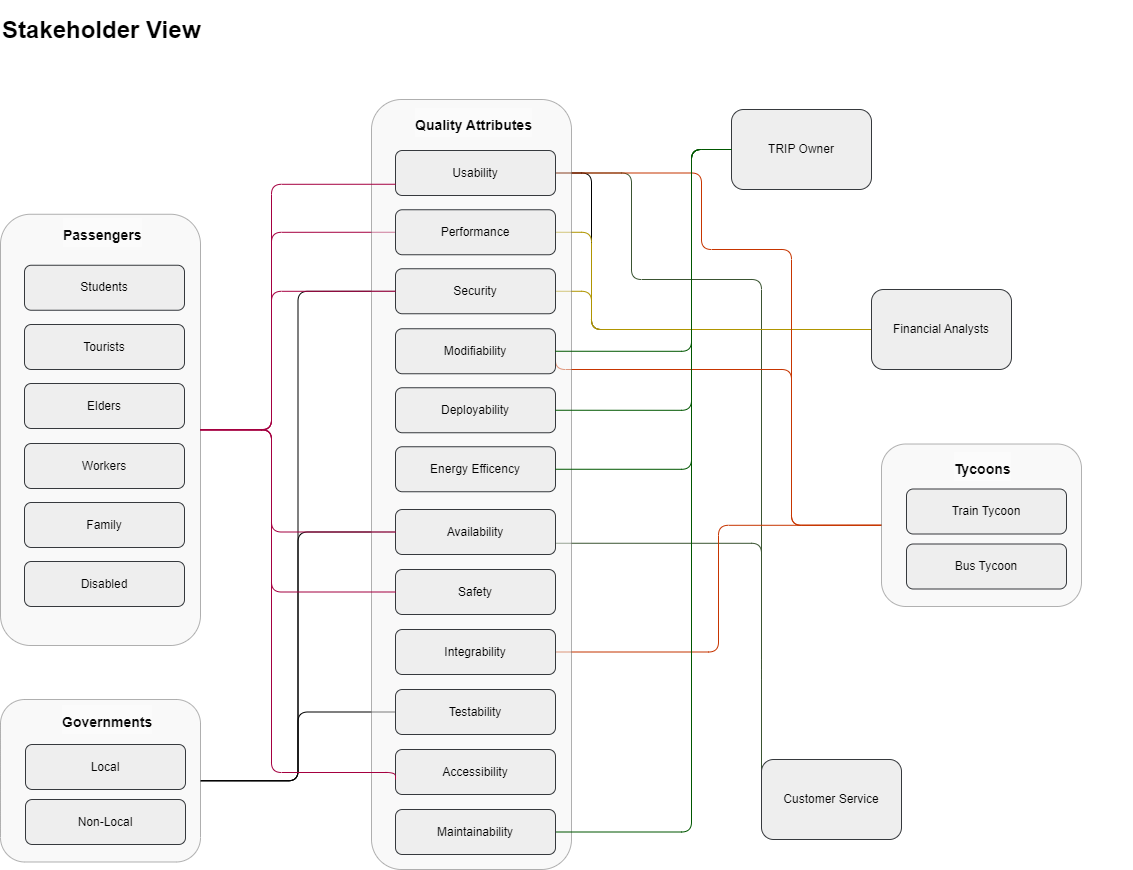
\includegraphics[width=\textwidth]{drawings/views_final_version/stakeholder_view.png}
    \caption{Stakeholder model of the TRIP system.}
    \label{fig:stakeholder_view_model}
\end{figure}

\subsection{Context Model}
\begin{figure}[H]
    \centering
    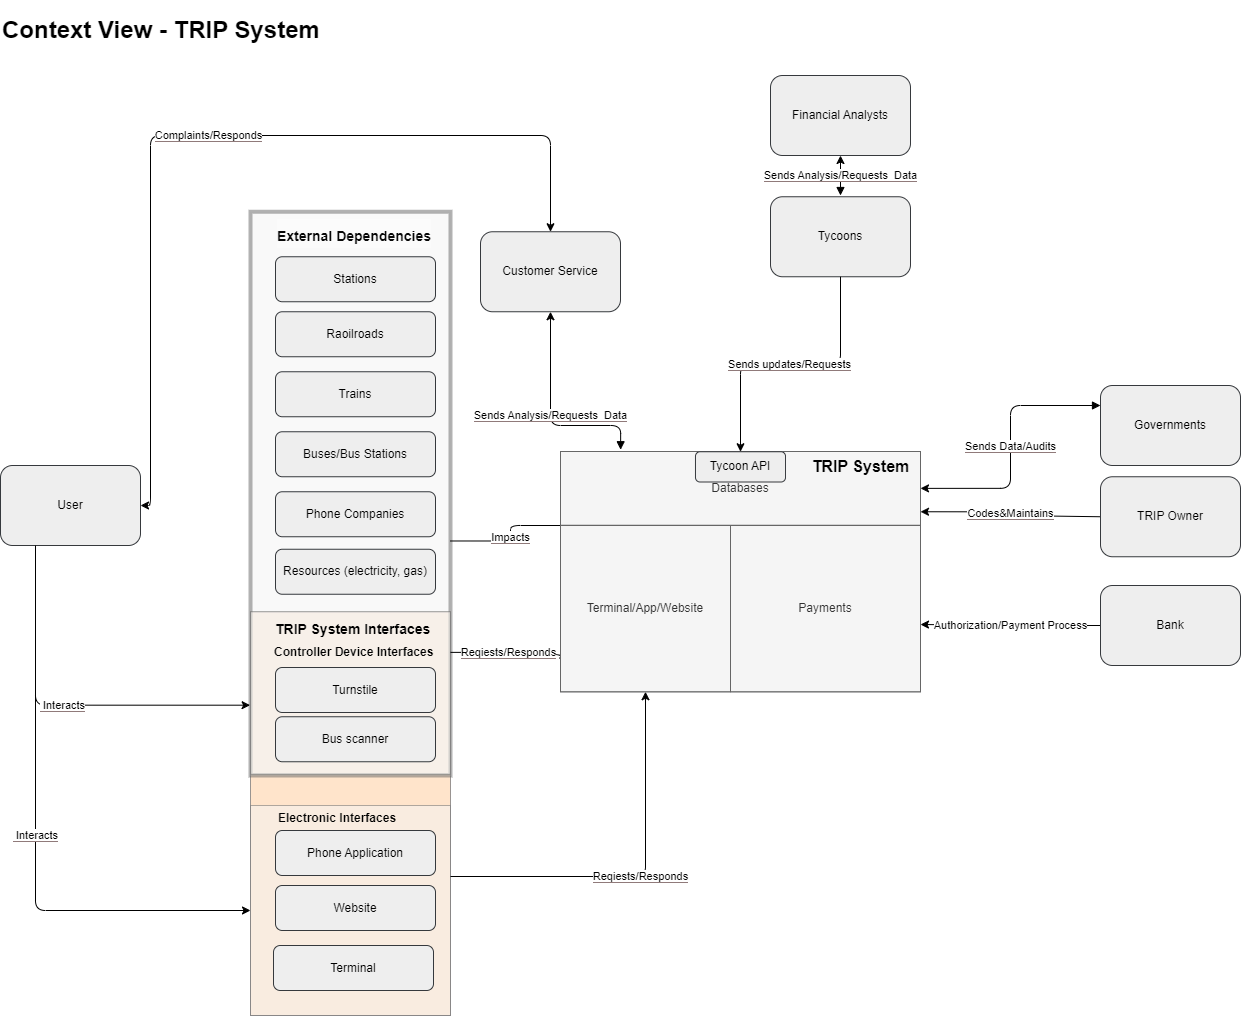
\includegraphics[width=\textwidth]{drawings/views_final_version/context_view.png}
    \caption{Context model of the TRIP system.}
    \label{fig:context_view_model}
\end{figure}

\begin{table}[H]
\centering
\begin{tabular}{@{}clp{9cm}@{}}
\toprule
\textbf{Id} & \textbf{Name} & \textbf{Description} \\
\midrule
1 & Passenger & Individuals who use the TRIP SYSTEM and its associated services, interacting through various interfaces. \\
2 & Customer Service & The department that handles passenger complaints and feedback, providing support and sending analysis or data requests to the system. \\
3 & Financial Analysts & Experts or entities that review financial data, requiring analytical information from the system for decision-making. \\
4 & Tycoons & The operational decision-makers of the system, possibly managers or algorithms that control system parameters and require data. \\
5 & Tycoon API & The programming interface through which Tycoons receive updates and send requests to the system. \\
6 & TRIP System & The core system that integrates various interfaces and processes, forming the central operation platform. \\
7 & Governments & Regulatory bodies that may require data or perform audits on the system for governance and compliance. \\
8 & TRIP Owner & The entity or person owning and maintaining the TRIP SYSTEM, responsible for its overall functionality. \\
9 & Bank & Financial institution that handles the authorization and processing of payments for the system. \\
10 & Stations & Locations where the TRIP SYSTEM provides service to passengers, such as train or bus stations. \\
11 & Railroads & Infrastructure providers that offer the tracks on which train services operate. \\
12 & Trains & The vehicles used by the system to transport passengers from one station to another. \\
13 & Buses/Bus Stations & The bus services and their stations that are part of the transport network. \\
14 & Phone Companies & Telecom service providers that facilitate mobile communication and data transfer for the system. \\
15 & Resources (electricity, gas) & Utility providers that supply essential power and energy required for the system’s operations. \\
16 & Controller Device Interfaces & The interfaces like turnstiles and bus scanners that manage access control and validate user credentials. \\
17 & Electronic Interfaces & Digital platforms such as mobile applications and websites that passengers interact with for services. \\
\bottomrule
\end{tabular}
\caption{Context model glossary for the TRIP System.}
\label{tab:glossary_context_view}
\end{table}


\section{Functional Viewpoint}
\begin{figure}[H]
    \centering
    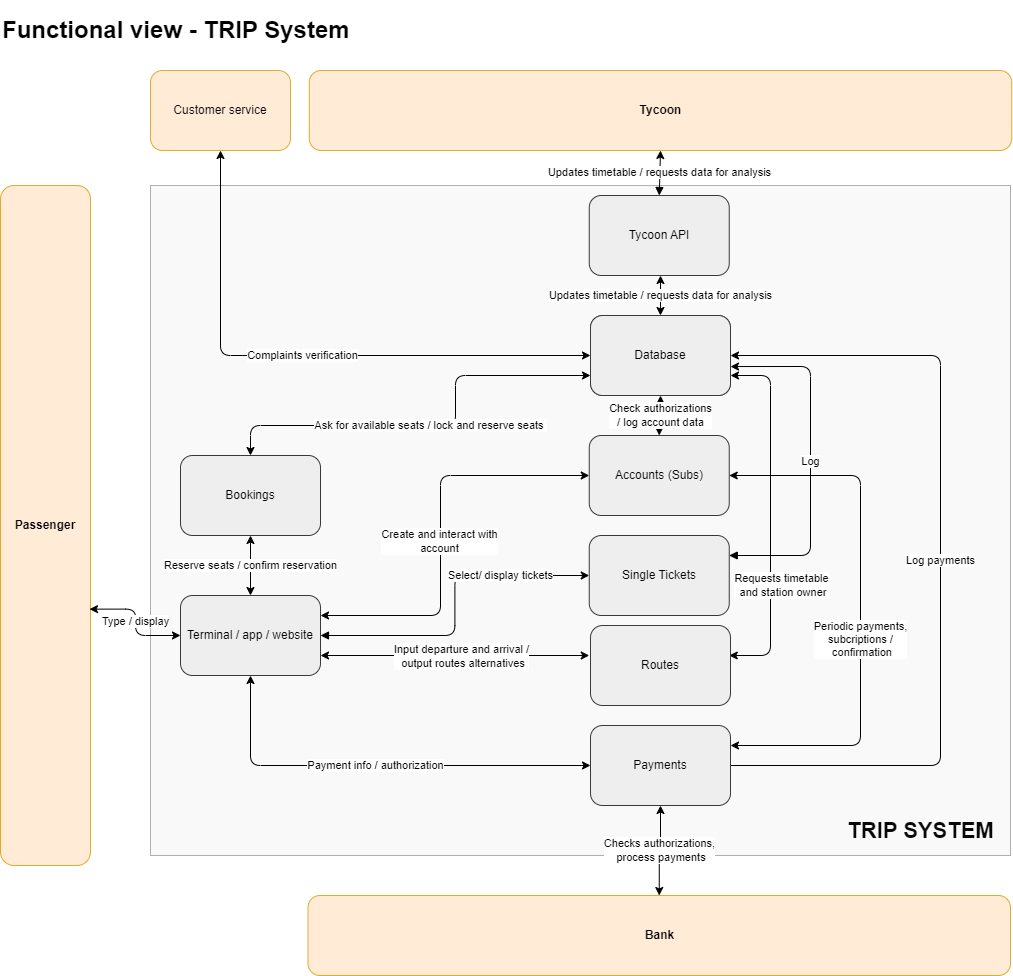
\includegraphics[width=\textwidth]{drawings/views_final_version/functional_view.png}
    \caption{TRIP System.}
    \label{fig:trip_system}
\end{figure}

\begin{table}[H]
    \centering
    \begin{tabular}{@{}clp{9cm}@{}}
    \toprule
    \textbf{Id} & \textbf{Name} & \textbf{Description} \\
    \midrule
    1 & Passenger & End-users of the TRIP SYSTEM who interact with various system components to manage their travel experience. \\
    2 & Customer Service & The interface for passengers to make inquiries or complaints and receive assistance with bookings or account issues. \\
    3 & Tycoon & The administrative or business logic module that updates timetables and analyzes system data for improvements or reporting. \\
    4 & Database & An abstraction for the set of databases that stores all system data including passenger accounts, bookings, and payment information. Detailed information about how different databases are handled is detailed in the Information View.\\
    5 & Bookings & The system component where passengers can inquire about seat availability and make reservations. \\
    6 & Accounts (Subs) & The system managing passenger accounts and subscriptions, responsible for authorization checks and account data logging. 
    It is is also responsible for single tickets and fillable cards, as they can be seen as temporary and anonymous accounts. \\
    7 & Routes & The component that manages route information and provides passengers with timetables, station ownership details, and route alternatives. \\
    8 & Payments & The module handling all financial transactions, including passenger payments and periodic billing. \\
    9 & Bank & The financial institution interface for authorizing and processing payments linked to the system. \\
    10 & Terminal/App/Website & User interfaces through which they can access services such as booking, route information, and payment. \\
    \bottomrule
    \end{tabular}
    \caption{Glossary of elements detailing the components of the TRIP SYSTEM and their roles in facilitating user interaction and service provision.}
    \label{tab:glossary_trip_system}
\end{table}

\begin{figure}[H]
    \centering
    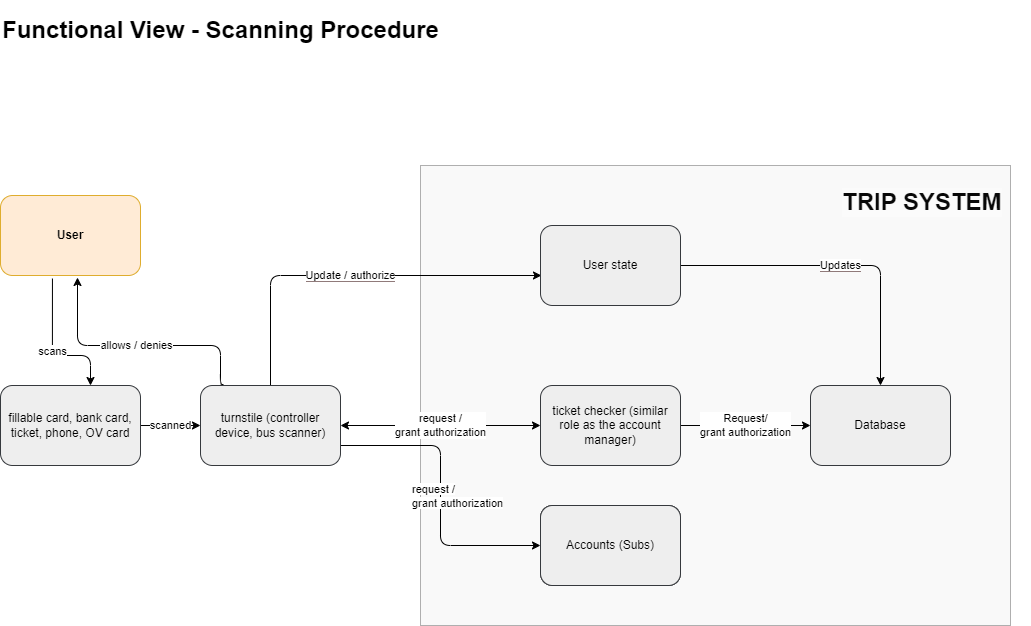
\includegraphics[width=\textwidth]{drawings/views_final_version/functional_view scanning.png}
    \caption{Interaction with a ticket scanner.}
    \label{fig:ticket_scanner}
\end{figure}

\begin{table}[H]
    \centering
    \begin{tabular}{@{}clp{9cm}@{}} % Adjust the width of the description column as needed to fit the page
    \toprule
    \textbf{Id} & \textbf{Name} & \textbf{Description} \\
    \midrule
    1 & Passenger & The individual who uses the trip system and interacts with various components such as turnstiles and ticket checkers. \\
    2 & Fillable Card, Bank Card, Ticket, Phone, OV Card & Various forms of identification or payment methods that the passenger can use within the system. These are scanned by the turnstile to allow or deny access. \\
    3 & Turnstile (Controller Device, Bus Scanner) & A physical barrier or scanner that reads the passenger's ticket or card and determines whether to grant or deny access based on the passenger state or account information. \\
    4 & Passenger State & A system component that maintains the current state of the passenger within the system, including authorization and access rights, which is updated upon passenger interaction with the turnstile. \\
    5 & Ticket Checker (Account Manager) & An agent or system role similar to the account manager that requests or grants authorization for passenger access, potentially by checking the passenger state against the database. \\
    6 & Accounts (Subs) & The subsystem managing passenger accounts and subscriptions, which may interact with the turnstile and ticket checker to verify and update passenger access rights. \\
    7 & Database & An abstraction for the set of databases that stores all system data including passenger accounts, bookings, and payment information. Detailed information about how different databases are handled is detailed in the Information View.\\
    \bottomrule
    \end{tabular}
    \caption{Glossary of elements for the Functional View - Turnstiles, detailing the components and their roles in passenger access and authorization within the TRIP SYSTEM.}
    \label{tab:glossary_turnstiles}
\end{table}

\section{Information Viewpoint}

\begin{figure}[H]
    \centering
    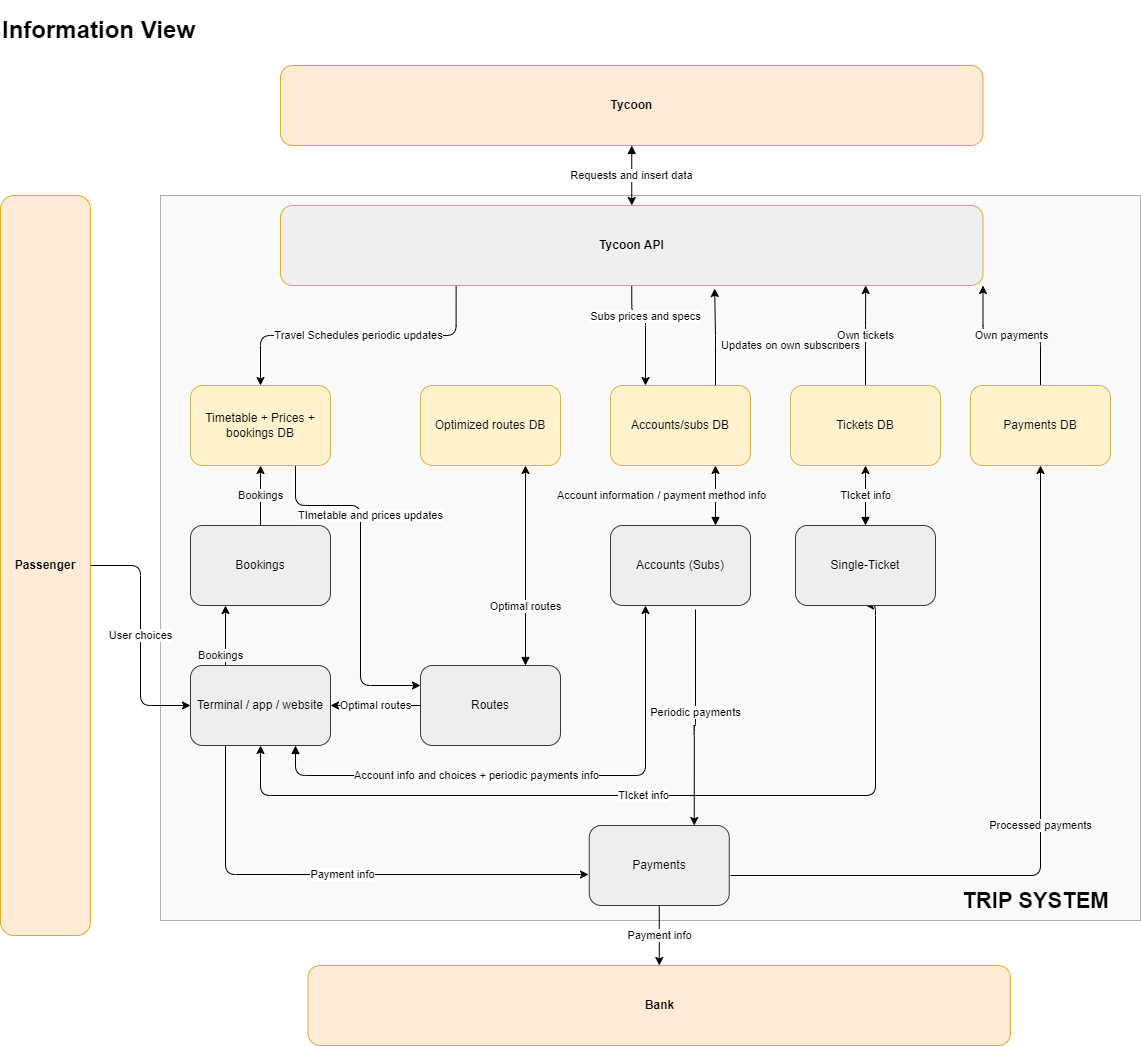
\includegraphics[width=\textwidth]{drawings/views_final_version/information_view.png}
    \caption{Information view.}
    \label{fig:information_view}
\end{figure}
\begin{table}[H]
    \centering
    \caption{Legend for the Information View of the TRIP SYSTEM.}
    \label{tab:information_view_legend}
    \begin{tabular}{@{}llp{10cm}@{}}
    \toprule
    \textbf{Id} & \textbf{Name} & \textbf{Description} \\
    \midrule
    1 & Timetable + Prices + Bookings DB & The database where travel schedules, prices, and booking details are stored. \\
    2 & Bookings & Interface for passengers to manage their booking requests and view current bookings. \\
    3 & Terminal / App / Website & Passenger interfaces for accessing booking, route, and payment information. \\
    4 & Routes & Component that contains information about the travel routes and helps in finding the optimal routes. \\
    5 & Optimized routes DB & Database storing the most efficient travel routes available. \\
    6 & Accounts/Subs DB & Database for managing passenger accounts and subscription details. \\
    7 & Tickets DB & Database where ticket purchases are recorded. \\
    8 & Payments DB & Database that records and processes payment transactions. \\
    9 & Accounts (Subs) & Management system for passenger accounts and subscriptions. \\
    10 & Single-Ticket & Interface for purchasing individual tickets. \\
    11 & Periodic payments & System handling regular subscription fee transactions. \\
    12 & Payments & System that processes immediate payment transactions. \\
    13 & Processed payments & Record of all completed payment transactions. \\
    \bottomrule
\end{tabular}
\end{table}

\begin{figure}[H]
    \centering
    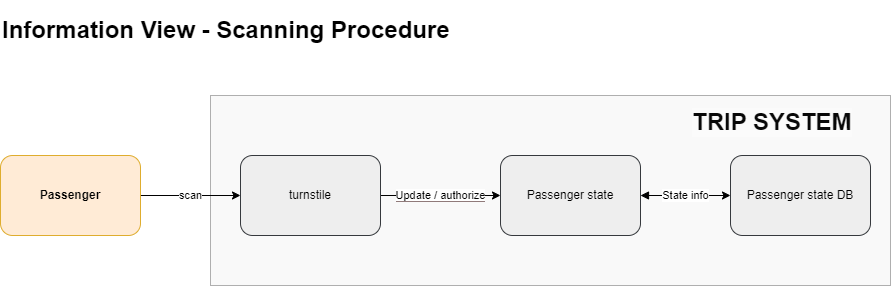
\includegraphics[width=\textwidth]{drawings/views_final_version/information_view scanning.png}
    \caption{Information view related to the scanning procedure.}
    \label{fig:information_view_scanning}
\end{figure}

\begin{table}[H]
    \centering
    \caption{Legend for the Scanning Procedure in the Information View of the TRIP SYSTEM.}
    \label{tab:scanning_procedure_legend}
    \begin{tabular}{@{}llp{10cm}@{}}
    \toprule
    \textbf{Id} & \textbf{Name} & \textbf{Description} \\
    \midrule
    1 & Passenger & The starting point representing the individual using the TRIP SYSTEM. \\
    2 & Turnstile & The physical or virtual entry point where the passenger scans to gain access. \\
    3 & Update / Authorize & The process that updates the system and authorizes the passenger to proceed. \\
    4 & Passenger State & The current status of the passenger within the system, which is updated after scanning. \\
    5 & Passenger State DB & The database that records the state information of the passenger. \\
    \bottomrule
\end{tabular}
\end{table}

\section*{Concurrency Viewpoint}

\section*{Development Viewpoint}

\section*{Deployment Viewpoint}